% !TEX root = main.tex
\documentclass[a4paper, UKenglish, 11pt]{uiomaster}
\usepackage{lipsum}
\usepackage[subpreambles=true]{standalone}
\usepackage[table,xcdraw]{xcolor}

\begin{document}

\chapter{Localizing Single Dipole Sources}

In this chapter we will present the results from training and performance of the neural networks presented in chapter 4. Section 1 deal with the results and discussion of the simple feed forward neural network, while section 2 will discuss how the alternative convolution neural network performe some of the same results.

\section{Localizing Single Dipole Sources}
% One example on coordinate prediction
% include the neural net that has been used

We begin by introducing the standard inverse problem for our neural network, DiLoc. In this context, the standard inverse problem refers to the task of predicting the x-, y-, and z-coordinates of dipole current sources responsible for generating measured EEG signals. The goal is to feed the network with EEG data corresponding to the electrical activity from randomly distributed dipoles in the cerebral cortex and have the network accurately output the locations of these current dipoles.

For this specific problem, the network demonstrates remarkable performance even without the use of L1 regularization. However, we include L2 penalty with a value of 0.5 to promote more generalizable solutions. The network is trained for 500 epochs, with each epoch completing in approximately 11.5 seconds. It is worth noting that the validation loss does not decrease significantly after approximately 350 epochs. As a result, fully training the network (for 350 epochs) would not require more than 4025 seconds, or roughly 1 hour and 7 minutes. Despite the validation loss stabilizing, we continued training for the full 500 epochs to ensure that there would be no further improvements in the validation data's performance. By training for a few more epochs beyond the point of loss stabilization, we could confirm that the network had reached its convergence and had effectively learned to generalize well on the given task.

Figure \ref{fig:single_dipole_accuracy} illustrates the network's loss as a function of training epochs. A clear trend of decreasing loss can be observed, indicating the network effectively learns the patterns in the data. The validation loss stabilizes around 350 epochs, while the training loss continues to decrease until a point between 400 and 500 epochs. Additionally, Figure \ref{fig:single_dipole_accuracy_targets} provides insight into the development of the validation loss for separate target coordinates plotted against training epochs. The figure most of all confirms that all separate target coordinates have been equally weighted, resulting in similar loss values for each of them. Moreover, it showcases that the small fluctuations in the loss, noticeable before 350 epochs, disappear beyond this threshold, indicating a stabilization of the loss for all three target coordinates.This observation aligns with the trend of the validation loss stabilizing at approximately 350 epochs as seen in the previously mentioned figure.


\begin{figure}[!htb]
    \centering
    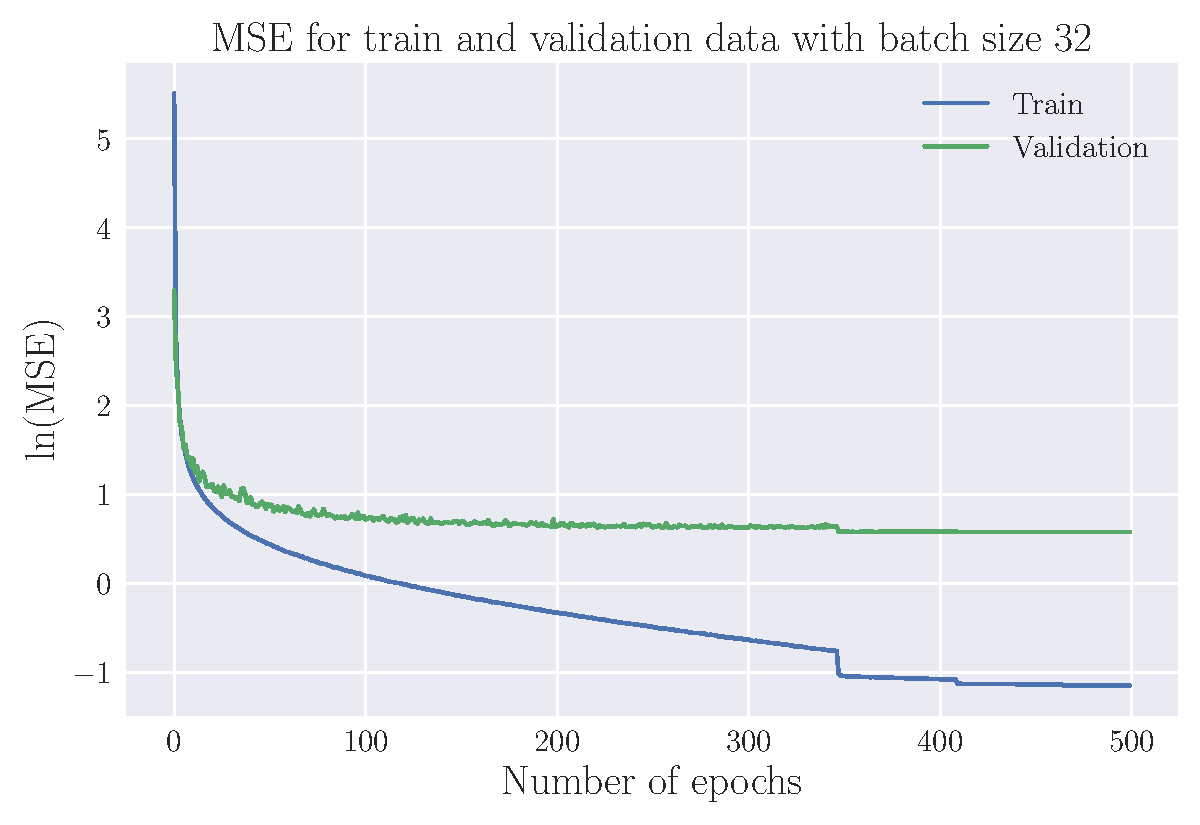
\includegraphics[width=\linewidth]{figures/mse_simple_32_0.001_0.35_0.5_0.0_500_(0).pdf}
    \caption{Training- and validation loss for DiLoc with 50 000 samples and tanh as activation function.}
    \label{fig:single_dipole_accuracy}
\end{figure}

\begin{figure}[!htb]
    \centering
    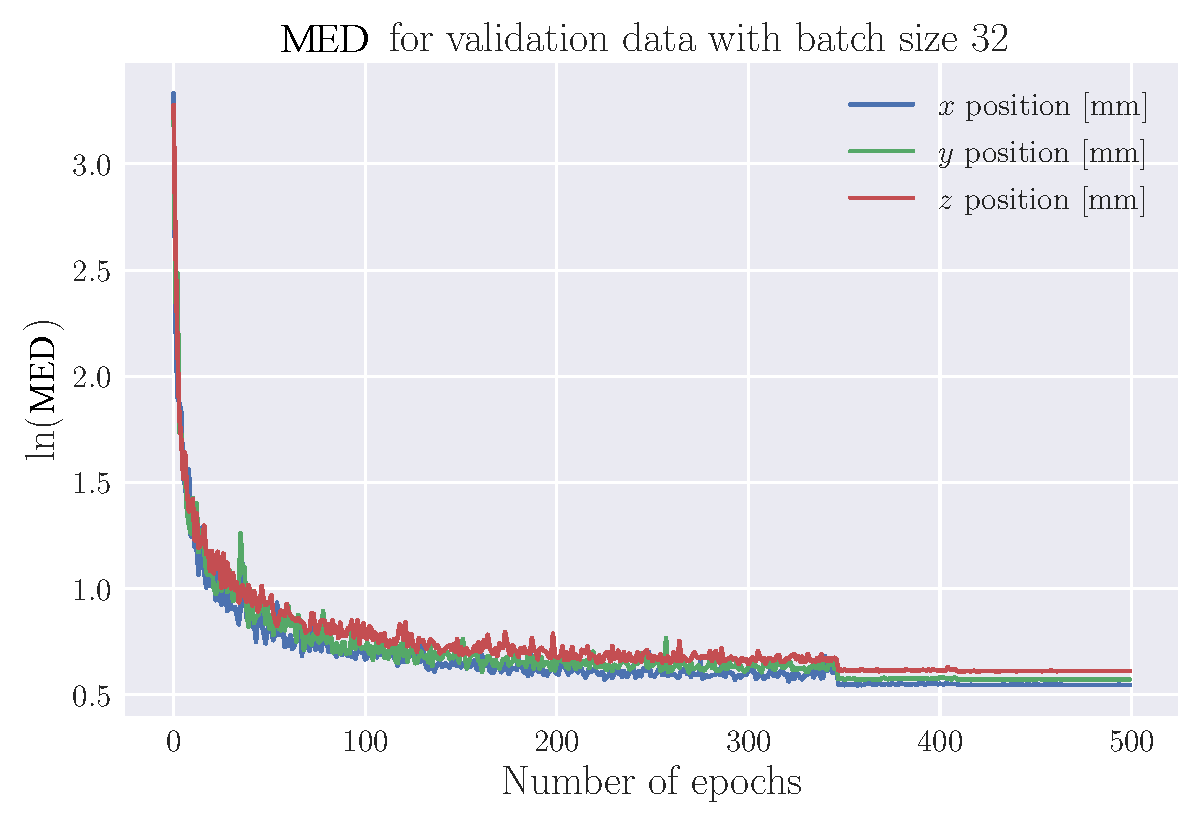
\includegraphics[width=\linewidth]{figures/mse_targets_simple_32_0.001_0.35_0.5_0.0_500_(0).pdf}
    \caption{Validation loss for the separate target values; the x-, y-, z-coordinate.}
    \label{fig:single_dipole_accuracy_targets}
\end{figure}


%\subsection{Performance Evaluation}

The DiLoc network's performance is evaluated using a variety of error metrics for the x-, y-, and z-coordinates. The x-coordinate ranges from -72 to 72 mm, the y-coordinate from -106 to 73 mm, and the z-coordinate from -52.66 to 81.15 mm.

Table \ref{table:error_simple_dipole} presents the results for the mean absolute error (MAE) in the DiLoc network's predictions. The MAE values for the x-, y-, and z-coordinates range from 0.645 mm to 0.678 mm. These findings indicate that, on average, the network's predictions exhibit an error smaller than 1 mm in each coordinate, showcasing a high level of accuracy. The MAE metric is robust and resilient to outliers, making it a suitable measure for assessing the network's general performance.

The mean squared error (MSE) values, ranging from 0.747 mm$^2$ to 0.824 mm$^2$, provide a measure of the average squared difference between the predicted and true values. Due to its squared nature, MSE penalizes outliers more significantly compared to MAE. Smaller MSE values signify improved performance, and all MSE values in our evaluation are below 1 mm$^2$. This observation highlights the network's remarkable precision, particularly when considering the broad range of coordinates involved. The small MSE values indicate the network's ability to provide accurate predictions even for data points that might be considered as "outliers," further demonstrating its robustness.

The root mean squared error (RMSE) values, ranging from 0.864 mm to 0.908 mm, represent the average magnitude of errors in the original units (mm). RMSE is the square root of MSE and is slightly higher than the corresponding MSE values, as taking the square root of numbers smaller than 1 results in slightly higher values. Nevertheless, all RMSE values are below 1 mm, further attesting to the network's exceptional accuracy. RMSE provides a measure of the standard deviation of errors around the mean and complements the MSE by assessing the spread of errors in the original units.

The error metrics for the Euclidean distance, derived from the three-dimensional space coordinates, are also calculated and presented in Table \ref{table:error_simple_dipole}. The values for MAE, MSE, and RMSE are smaller than 1 mm, indicating accurate predictions by the DiLoc network for the inverse problem. The performance metrics for the Euclidean distance corroborate the network's ability to predict the dipole location with a high level of precision and accuracy.

It is worth mentioning that among the three coordinates, the z-coordinate exhibits the highest error values. This observation suggests that the DiLoc network encounters more challenges in accurately predicting the z-coordinate of the dipole source. One plausible explanation for this discrepancy could be attributed to the nature of the inverse problem, where EEG patterns for dipole sources do not produce significant changes in the pattern of electrical potential recording, but rather in magnitude. Additionally, the smaller representation of z-values compared to x- and y-coordinates could contribute to the consistent larger errors in the z-direction. However, despite these challenges, the overall error metrics indicate that the DiLoc network is capable of predicting the dipole location with a reasonable level of accuracy, signifying its practical viability for real-world applications.



% Please add the following required packages to your document preamble:
% \usepackage[table,xcdraw]{xcolor}
% If you use beamer only pass "xcolor=table" option, i.e. \documentclass[xcolor=table]{beamer}
\begin{table}[!htb]
\begin{tabular}{l|cccc|}
\cline{2-5}
\rowcolor[HTML]{CBCEFB}
\cellcolor[HTML]{FFFFFF}                           & \multicolumn{4}{c|}{\cellcolor[HTML]{CBCEFB}{\color[HTML]{000000} \textbf{Error for different target values}}}                                                                                                                                                                                                                                                                                                                                                     \\ \cline{2-5}
\rowcolor[HTML]{EFEFEF}
\cellcolor[HTML]{FFFFFF}\textbf{}                  & \multicolumn{1}{l|}{\cellcolor[HTML]{EFEFEF}\begin{tabular}[c]{@{}l@{}}x-coordinate\\ {[}mm{]}\end{tabular}} & \multicolumn{1}{l|}{\cellcolor[HTML]{EFEFEF}\begin{tabular}[c]{@{}l@{}}y-coordinate \\ {[}mm{]}\end{tabular}} & \multicolumn{1}{l|}{\cellcolor[HTML]{EFEFEF}\begin{tabular}[c]{@{}l@{}}z-coordinate \\ {[}mm{]}\end{tabular}} & \multicolumn{1}{l|}{\cellcolor[HTML]{EFEFEF}\begin{tabular}[c]{@{}l@{}}Euclidean \\ Distance {[}mm{]}\end{tabular}} \\ \hline
\multicolumn{1}{|l|}{\cellcolor[HTML]{EFEFEF}MAE}  & \multicolumn{1}{c|}{0.645}                                                                                  & \multicolumn{1}{c|}{0.665}                                                                                   & \multicolumn{1}{c|}{0.678}                                                                                   & 0.662                                                                                                              \\ \hline
\multicolumn{1}{|l|}{\cellcolor[HTML]{EFEFEF}MSE}  & \multicolumn{1}{c|}{0.747}                                                                                  & \multicolumn{1}{c|}{0.775}                                                                                   & \multicolumn{1}{c|}{0.824}                                                                                   & 0.782                                                                                                              \\ \hline
\multicolumn{1}{|l|}{\cellcolor[HTML]{EFEFEF}RMSE} & \multicolumn{1}{c|}{0.864}                                                                                  & \multicolumn{1}{c|}{0.880}                                                                                   & \multicolumn{1}{c|}{0.908}                                                                                   & 0.884                                                                                                              \\ \hline
\end{tabular}
\caption{\textbf{Evaluation of the DiLoc performance utializing different Error Metrics.} \newline
Network performance on test dataset consisting of 20000 samples. The errors are measured using Mean Squared Error (MSE), Mean Absolute Error (MAE), and Root Mean Squared Error (RMSE).}
\label{table:error_simple_dipole}
\end{table}


In order to conduct a detailed analysis of the network's performance, Figure \ref{fig:MAE_crossections} presents the Mean Squared Error (MSE) for various dipole locations within the New York head model cortex matrix. The figure provides valuable insights into the distribution of errors across different regions of the cortex, with three cross-sections—front, top, and side—depicted for examination. It is important to note that these cross-sections include data points from the training, validation, and test datasets, making these results indicative of the network's overall performance rather than real-world scenarios. However, the analysis aims to examine the distribution of errors and identify potential areas where the network's performance may be weaker, helping to gain valuable insights into its predictive capabilities.

The MSE values presented in the panels are consistently below 1 mm, which indicates a high level of accuracy in the network's predictions. These results are promising and demonstrate the network's ability to estimate dipole locations with a high level of precision. The panels also offer an opportunity to assess whether the network performs differently for dipoles located in the gyrus compared to the sulcus.

Initially, it might be assumed that EEG signals originating from dipoles in the sulcus present greater challenges for the network's analysis and prediction. This assumption is based on the deeper placement of dipoles within the sulcus compared to those in the gyrus, as well as the potential complexities introduced by the dipole's orientation within the cortex. However, upon closer examination of Figure \ref{fig:MAE_crossections}, it becomes evident that the distribution of MSE values does not exhibit a clear correlation with the brain's structural characteristics. The MSE values appear to vary randomly across different regions, indicating that the network's performance is not significantly influenced by the distinction between the gyrus and sulcus.

Surprisingly, the Mean Squared Error (MSE) for all data points where dipoles are located in sulci is reported to be 1.283 mm, which is even smaller than for dipoles in the gyrus, where the MSE measures 1.349 mm. This observation challenges the initial assumption and indicates that the network demonstrates exceptional accuracy in predicting dipole locations, irrespective of their placement within the cortex. The small Mean Absolute Error (MAE) values further underscore the network's remarkable capacity to effectively capture the intricate features and variations associated with deeper cortical placements. These findings not only attest to the network's robustness but also reinforce its potential for precise dipole localization within the human brain across different cortical structures.

Furthermore, the figures reveal a noticeable concentration of data points with red and yellow marks, indicating higher Mean Squared Error (MSE) values, in the deeper locations within the cortex. This observation partially aligns with the slightly higher error values for the z-coordinate, as presented in Table \ref{table:error_simple_dipole}, and is consistent with the theory related to the nature of the inverse problem. According to this theory, EEG patterns for dipole sources do not cause substantial changes in the pattern of electrical potential recording; instead, they primarily influence the magnitude of the signals. The presence of higher MSE values in deeper regions might be attributed to the decreasing signal-to-noise ratio of EEG signals originating from these cortical areas.

In conclusion, the detailed analysis of the network's performance through cross-sectional representations provides valuable insights into its predictive capabilities. The consistently low MSE values across different cortical regions demonstrate the network's remarkable accuracy in estimating dipole locations. Moreover, the absence of a clear correlation between MSE values and brain structural characteristics suggests that the network performs robustly across diverse cortical structures. These results have significant implications for the network's potential clinical and research applications, as it showcases its ability to accurately predict dipole locations within the human brain, regardless of their depth and orientation within the cortex.



\begin{figure}[!htb]
    \centering
    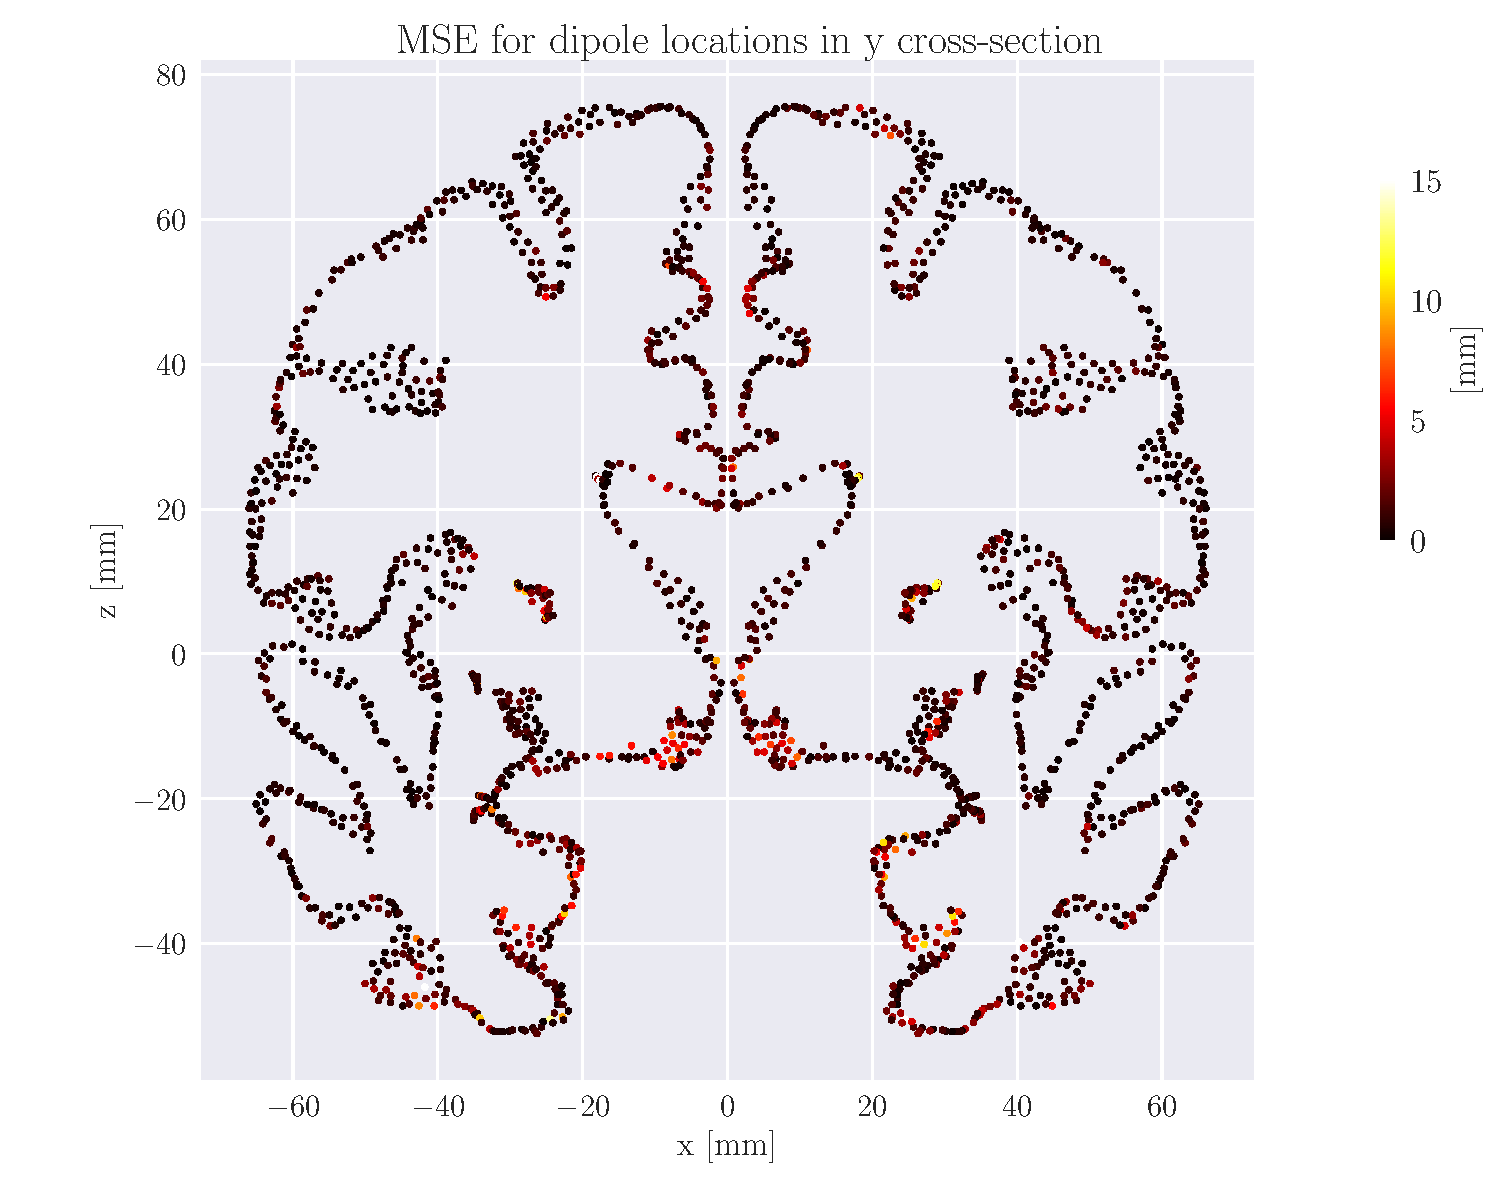
\includegraphics[width=0.7\linewidth]{figures/NEW_simple_dipole_error_Euclidean Distance_00.pdf}
    \vspace{10pt} % Adjust the vertical spacing between the images
    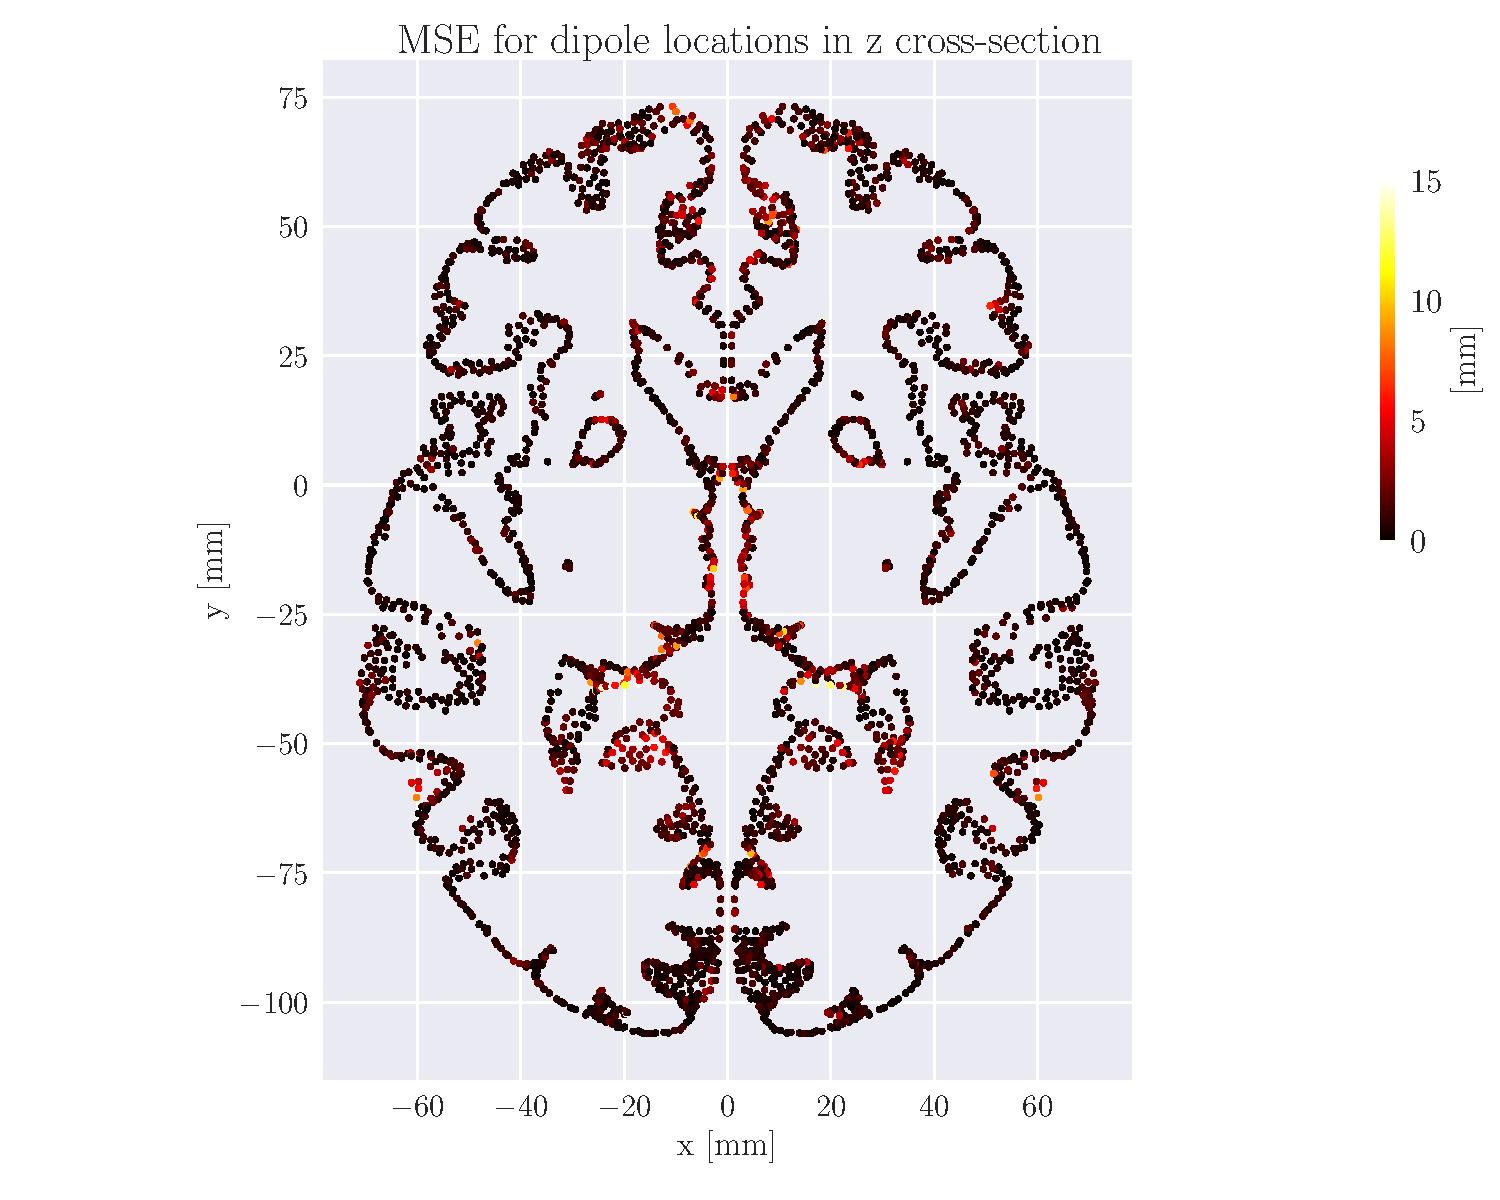
\includegraphics[width=0.7\linewidth]{figures/NEW_simple_dipole_error_Euclidean Distance_10.pdf}
    \vspace{10pt} % Adjust the vertical spacing between the images
    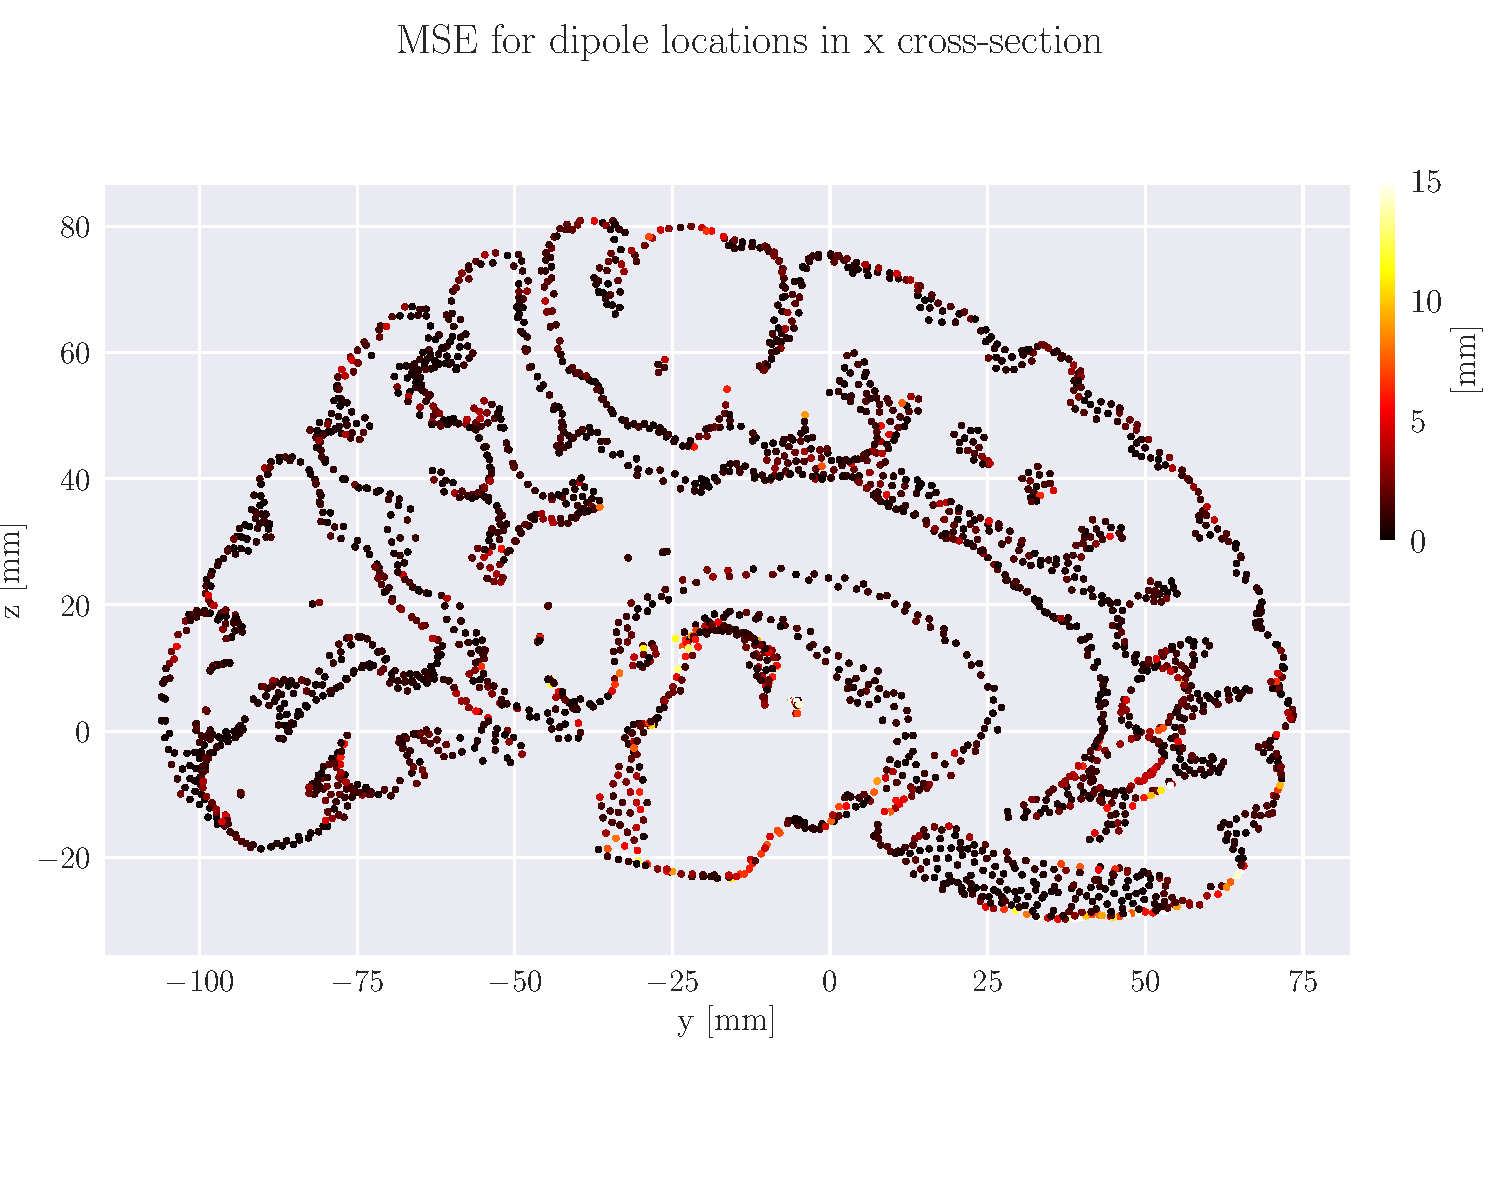
\includegraphics[width=0.7\linewidth]{figures/NEW_simple_dipole_error_Euclidean Distance_20.pdf}
    \caption{Different cross-sections of the cortex from the New York head model, seen from front, top and side. Each point represents a possible position in the cortex matrix. The color of the each point indicates the mean absolute error (MAE) of the neural network when predicting that specific dipole location.}
    \label{fig:MAE_crossections}
\end{figure}



\section{Convolution Neural Network Approach for localizing single dipole sources}

Some results for the prediction of location for single current dipoles.


\begin{figure}[!htb]
\centering
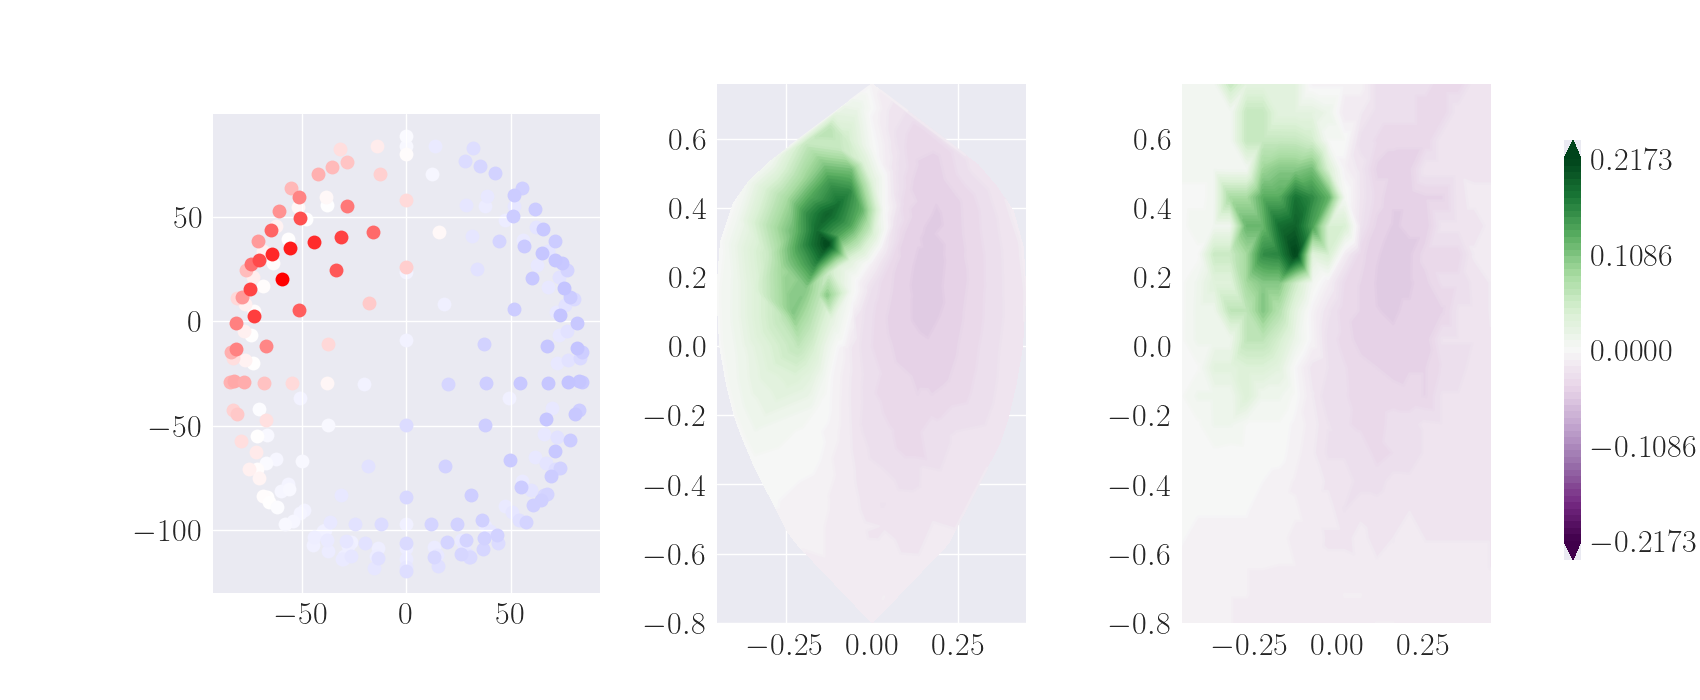
\includegraphics[width=\linewidth]{../Code/plots/finals/new_eeg_dipole_pos_0.png}
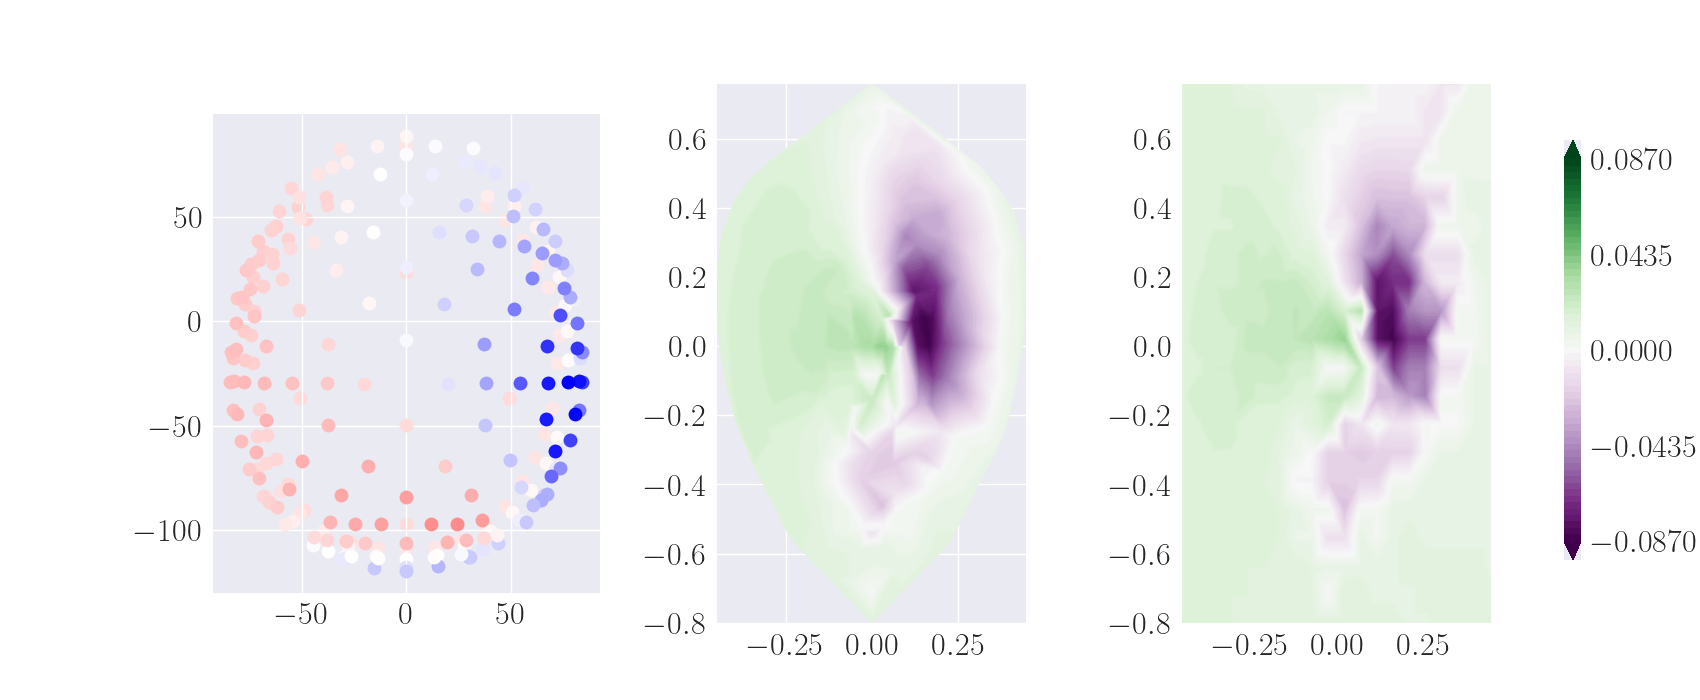
\includegraphics[width=\linewidth]{../Code/plots/finals/new_eeg_dipole_pos_4.png}
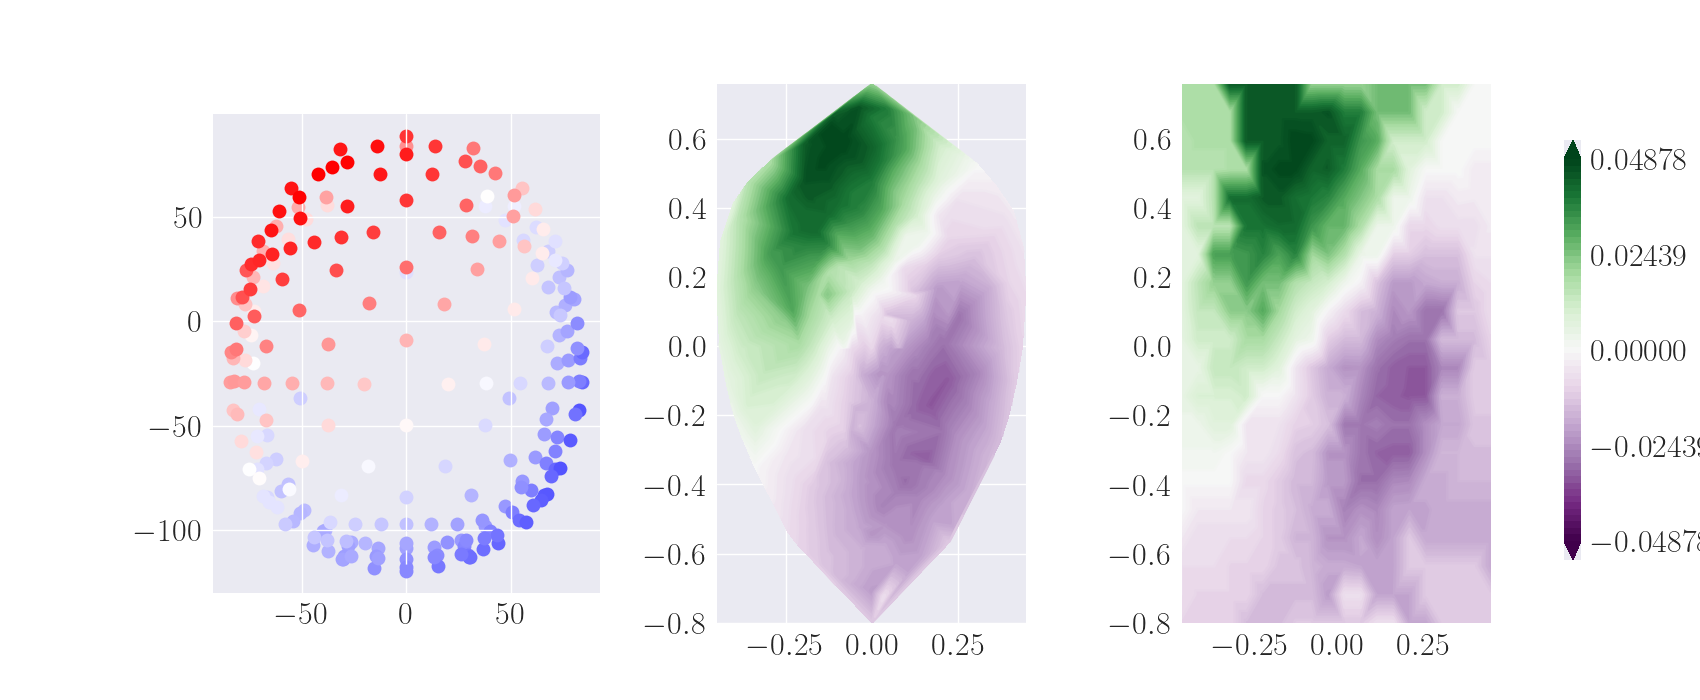
\includegraphics[width=\linewidth]{../Code/plots/finals/new_eeg_dipole_pos_6.png}

\caption{\newline
\textbf{Right}: EEG measure for 3 different samples measured in $\mu V$. \newline
\textbf{Middle and Left}: Illustration of the interpolation of the EEG data into two-dimensional matrix.}
\label{fig:eeg_dipole_pos_0}

\end{figure}

\begin{figure}[!htb]
    \centering
    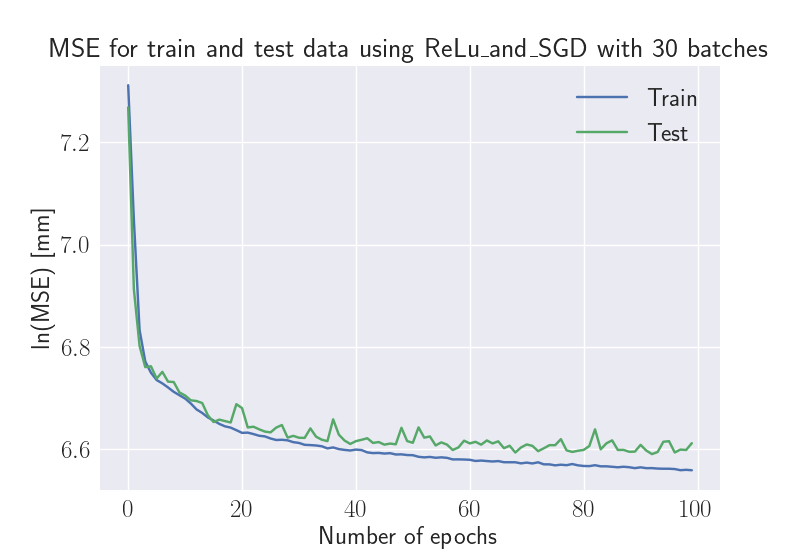
\includegraphics[width=\linewidth]{../Code/plots/finals/MSE_CNN_dipoles_2_interpolated_CNN_20x20_10000_ReLu_and_SGD_30_100.png}
    \caption{The validation accuracy for Convolutional Neural Network with 10 000 samples (20x20 matrix) with ReLU activation function. }
    \label{fig:single_dipole_accuracy_CNN_2d}
\end{figure}

% \begin{figure}[!htb]
%     \centering
%     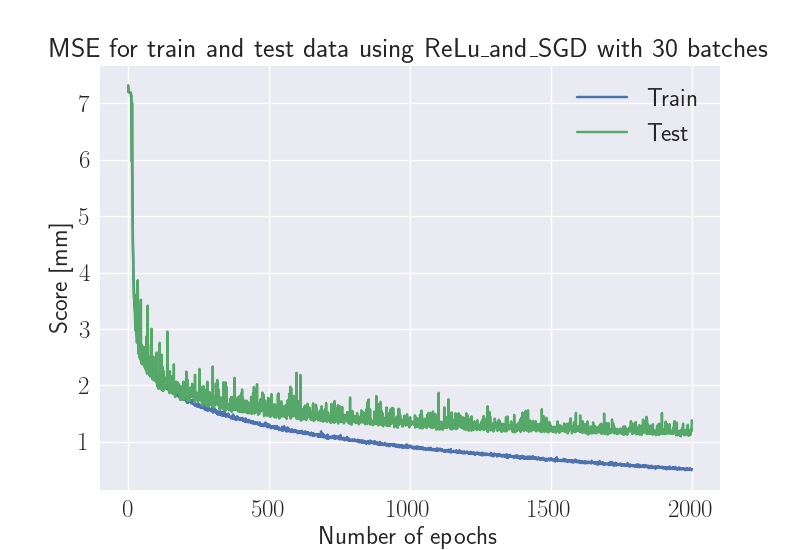
\includegraphics[width=\linewidth]{../Code/plots/CNN/MSE_interpolated_CNN_20x20_10000_ReLu_and_SGD_30_2000.png}
%     \caption{The validation accuracy for Convolutional Neural Network with 10 000 samples (20x20 interpolated matrix) with ReLU activation function. }
%     \label{fig:single_dipole_accuracy_CNN}
% \end{figure}


\end{document}
